\documentclass[../AnalysisNoteJBuxton.tex]{subfiles}
\begin{document}

\subsection{Cascade Reconstruction}
\label{CascadeReconstruction}

Our motivation for studying $\Xi$K$^{\pm}$ systems is to hopefully better understand the striking difference in the $\Lambda$K$^{+}$ and $\Lambda$K$^{-}$ data at low $k^{*}$ (Figure \ref{fig:cLamcKchCfs0010}).

The reconstruction of $\Xi$ particles is one step above V0 reconstruction.  V0 particles are topologically reconstructed by searching for the charged daughters' tracks into which they decay.  With $\Xi$ particles, we search for the V0 particle and charged daughter into which the $\Xi$ decays.  In the case of $\Xi^{-}$, we search for the $\Lambda$ (V0) and $\pi^{-}$ (track) daughters.  We will refer to this $\pi$ as the ``bachelor $\pi$".

The following cuts were used to select good $\Xi^{-}$ ($\bar{\Xi}^{+}$) candidates:

\begin{enumerate}
 \item V0 Daughter Reconstruction
 \begin{enumerate}
  \item V0 Daughter Particle Cuts
   \begin{enumerate}
    \item{Cuts Common to Both Daughters}
    \begin{enumerate}
     \item $|\eta| < 0.8$
     \item SetTPCnclsDaughters(80)
     \item SetStatusDaughters(AliESDtrack::kTPCrefic)
     \item SetMaxDcaV0Daughters(0.4)
    \end{enumerate}
    \item Pion Specific Daughter Cuts 
    \begin{enumerate}
     \item $p_{T} > 0.16$
     \item DCA to prim vertex $>$ 0.3
    \end{enumerate}
    \item Proton Specific Daughter Cuts
    \begin{enumerate}
     \item $p_{T} > $ 0.5($p$) [0.3($\bar{p}$)] GeV/\textit{c}
     \item DCA to prim vertex $>$ 0.1 
    \end{enumerate}
   \end{enumerate}
  \item V0 Cuts  
  \begin{enumerate}
   \item $|\eta| < 0.8$
   \item $p_{T} > 0.4$ GeV/\textit{c}
   \item $|m_{inv} - m_{PDG}| <$ 3.8 MeV
   \item DCA to prim. vertex $>$ 0.2 cm   
   \item Cosine of pointing angle to $\Xi$ decay vertex $>$ 0.9993
   \item OnFlyStatus = false
   \item Decay Length $<$ 60 cm
   \item The misidentification cuts described in Section \ref{LambdaReconstruction} are utilized 
  \end{enumerate} 
 \end{enumerate}
 \item Bachelor $\pi$ Cuts
 \begin{enumerate}
  \item $|\eta| < 0.8$
  \item $p_{T} < 100$ GeV/\textit{c}
  \item DCA to prim vertex $>$ 0.1 cm
  \item SetTPCnclsDaughters(70)
  \item SetStatusDaughters(AliESDtrack::kTPCrefic)
 \end{enumerate}
 \item $\Xi$ Cuts
 \begin{enumerate}
  \item $|\eta| < 0.8$
  \item $0.8 < p_{T} < 100$ GeV/\textit{c}
  \item $|m_{inv} - m_{PDG}| <$ 3.0 MeV
  \item DCA to prim. vertex $<$ 0.3 cm
  \item Cosine of pointing angle $>$ 0.9992
 \end{enumerate}
 
 
 \item Shared Daughter Cut for $\Xi$ Collection
 \begin{itemize}
  \item Iterate through $\Xi$ collection to ensure that no daughter is used in more than one $\Xi$ candidate
 \end{itemize} 
 
\end{enumerate}




\begin{figure}[h]
  \centering
  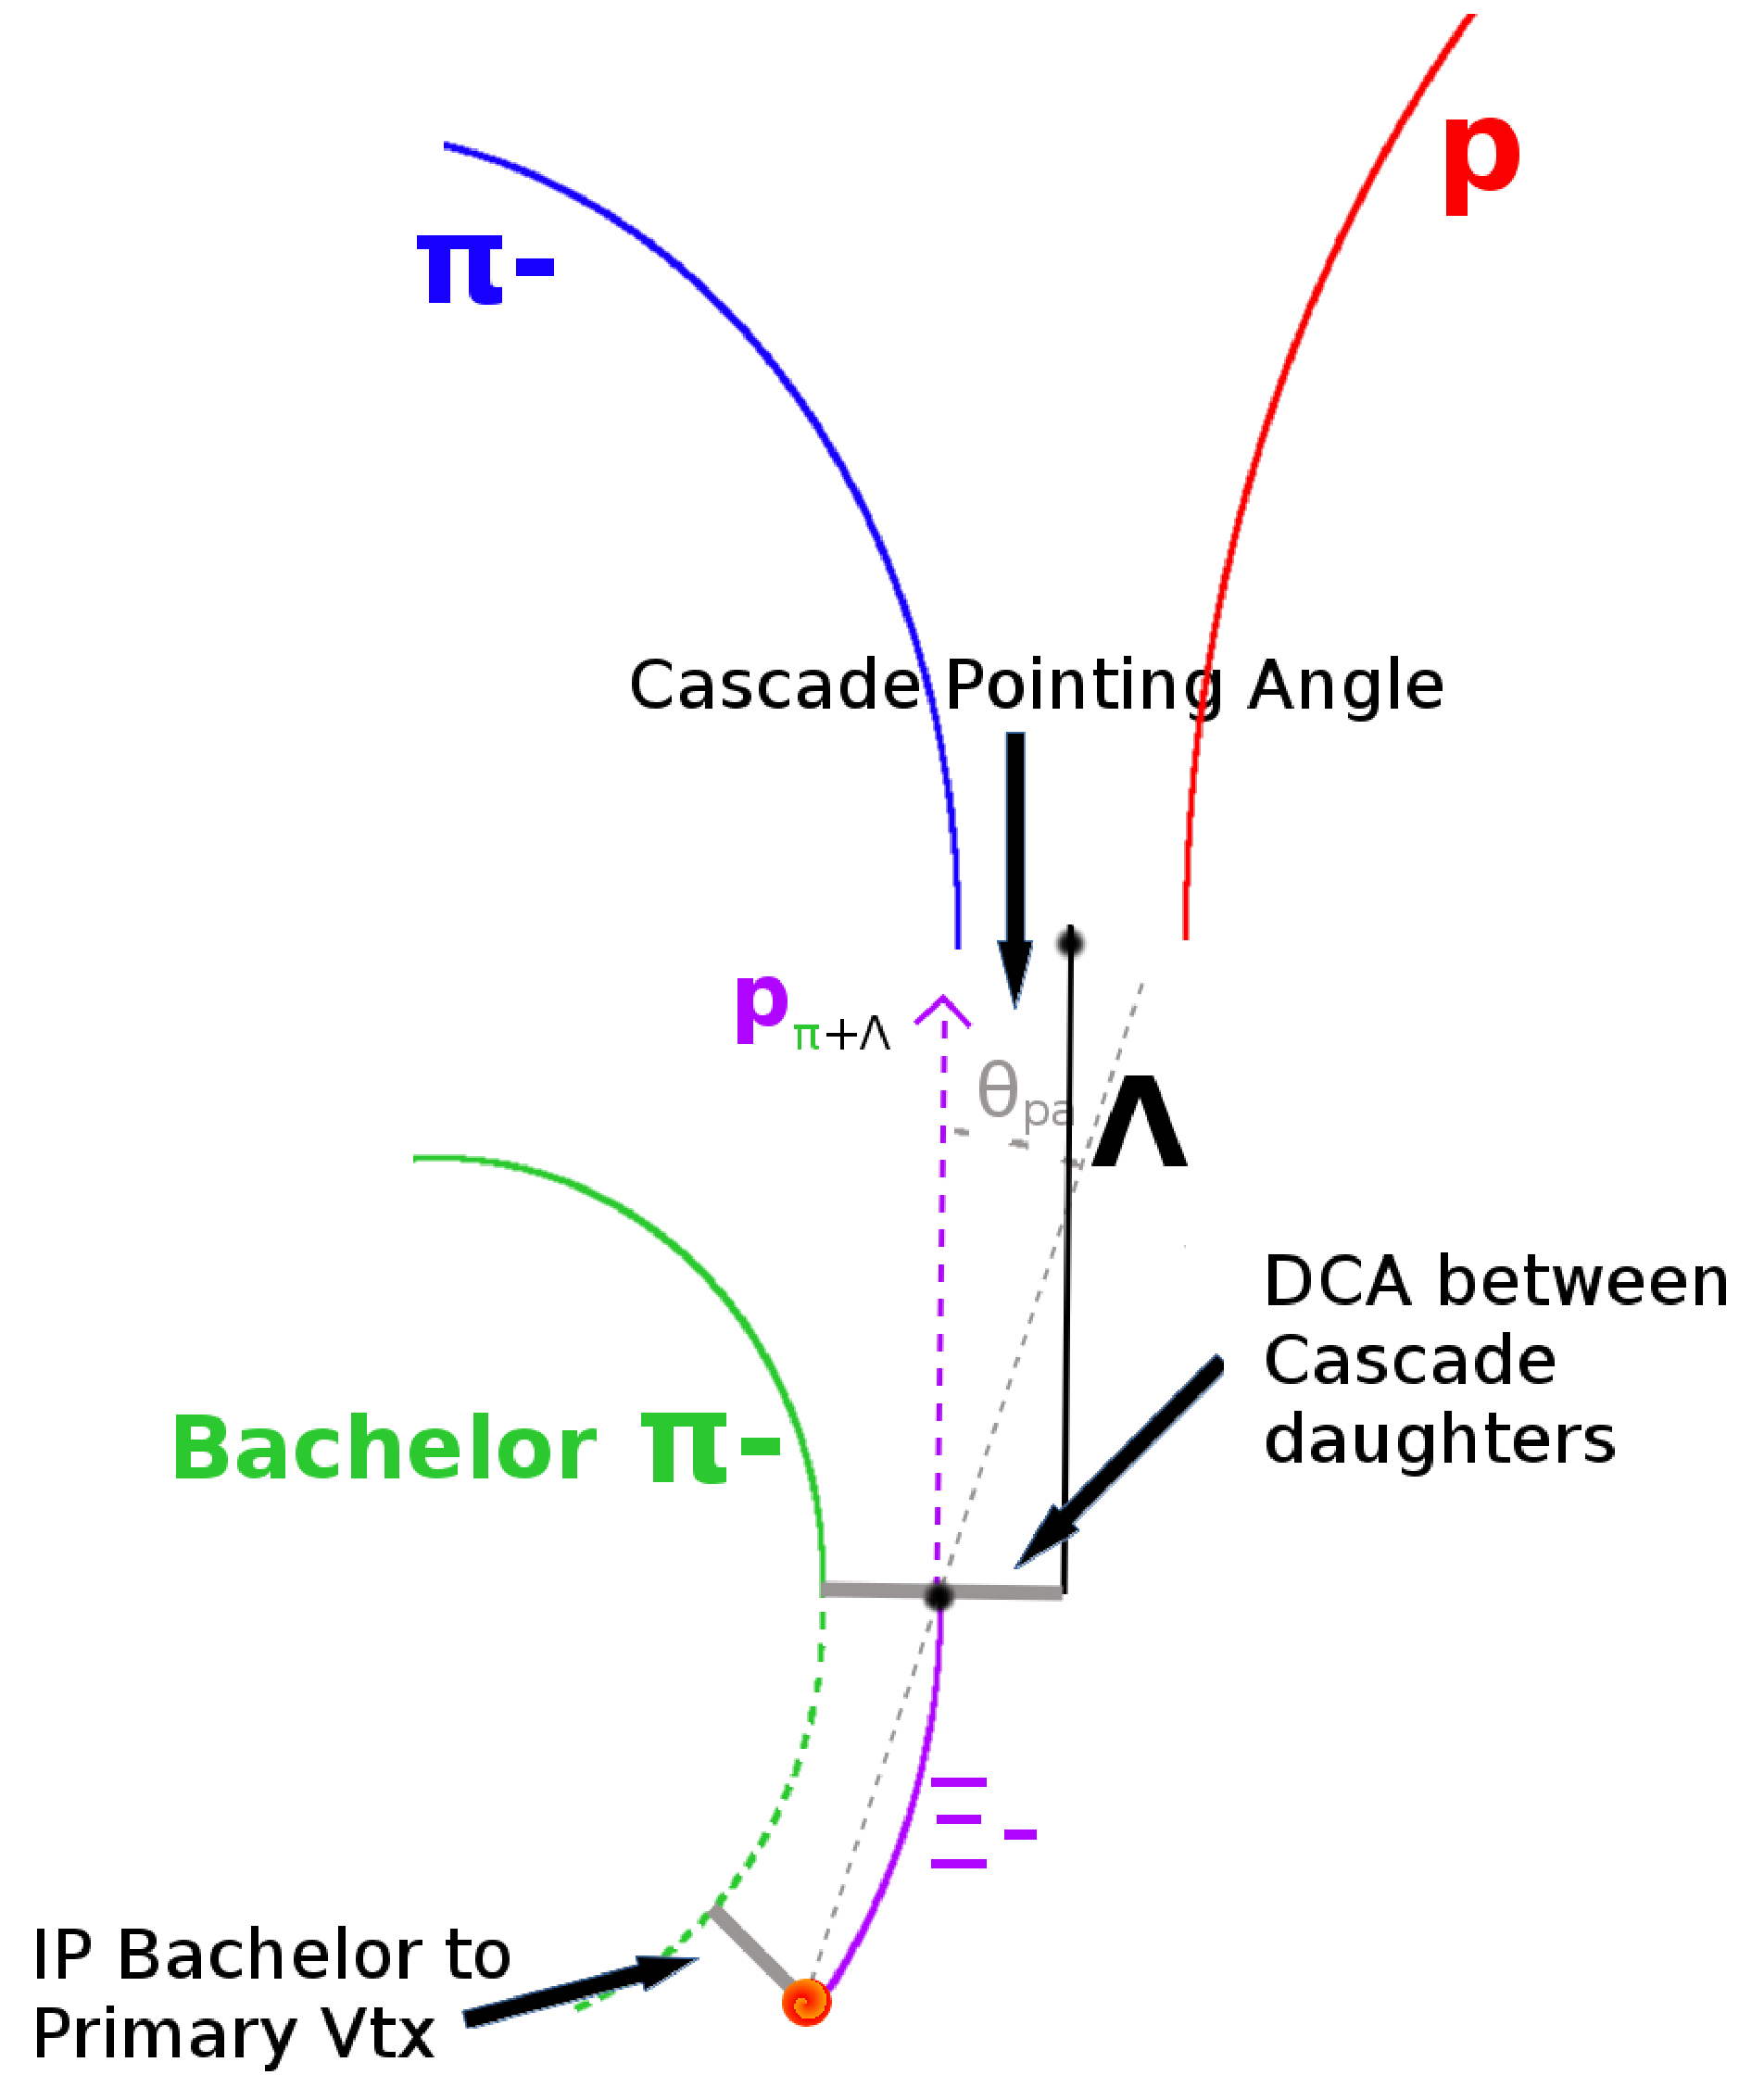
\includegraphics[width=0.5\textwidth]{3_DataSelection/Figures/XiCuts.pdf}
  \caption[$\Xi$ Reconstruction]{$\Xi$ Reconstruction}
  \label{fig:XiReconstruction}
\end{figure}

The purity of our $\Xi$ and $\bar{\Xi}$ collections are calculated just as those of our V0 collections \ref{V0Selection}.
Figure \ref{fig:XiPurity}, which is used to calculate the purity, shows the m$_{inv}$ distribution of our $\Xi$($\bar{\Xi}$) candidates just before the final m$_{inv}$ cut.  Currently, we have Purity($\Xi^{-}$) $\approx$ 90\% and Purity($\bar{\Xi}^{+}$) $\approx$ 92\%.

\begin{figure}[h!]
  \centering
  %%----start of first subfigure---  
  \subfloat[$\Xi^{-}$ Purity]{
    \label{fig:XiPurity:a}
    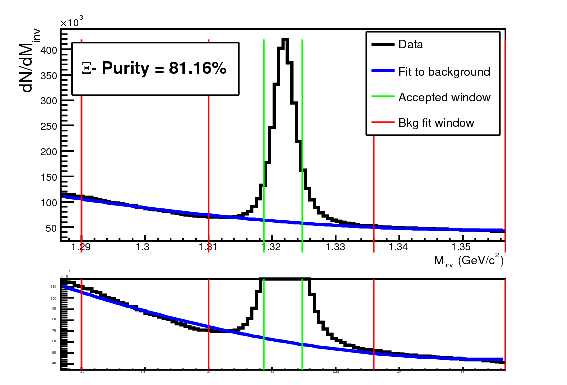
\includegraphics[width=0.49\textwidth]{3_DataSelection/Figures/XiPurity_XiKchP.pdf}}
  %%----start of second subfigure---
  \subfloat[$\bar{\Xi}$ Purity]{
    \label{fig:XiPurity:b}
    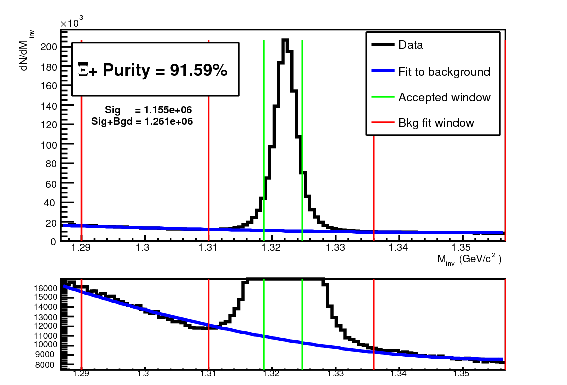
\includegraphics[width=0.49\textwidth]{3_DataSelection/Figures/AXiPurity_AXiKchP.pdf}}
  %%----overall caption----
  \caption[$\Xi^{-}$($\bar{\Xi}^{+}$) Purity]{$\Xi^{-}$($\bar{\Xi}^{+}$) Purity 0-10\%:  Purity($\Xi^{-}$) $\approx$ 90\% and Purity($\bar{\Xi}^{+}$) $\approx$ 92\%.}
  \label{fig:XiPurity}
\end{figure}

\end{document}